\section{Auswertung}
\label{sec:Auswertung}
Im folgenden sind alle Amplituden in willkürlichen Einheiten angegeben.
\subsection{Vorbereitendes Experiment}
Um Redundanz zu vermeiden sind statt alle zwölf nur die Frequenzspektren, wo der Zylinder die Länge $\qty{50}{\milli\meter}$ und $\qty{600}{\milli\meter}$ hat, in der Abbildung
\ref{fig:os} aufgeführt.
\begin{figure}
\begin{subfigure}{0.48\textwidth}%
\centering%
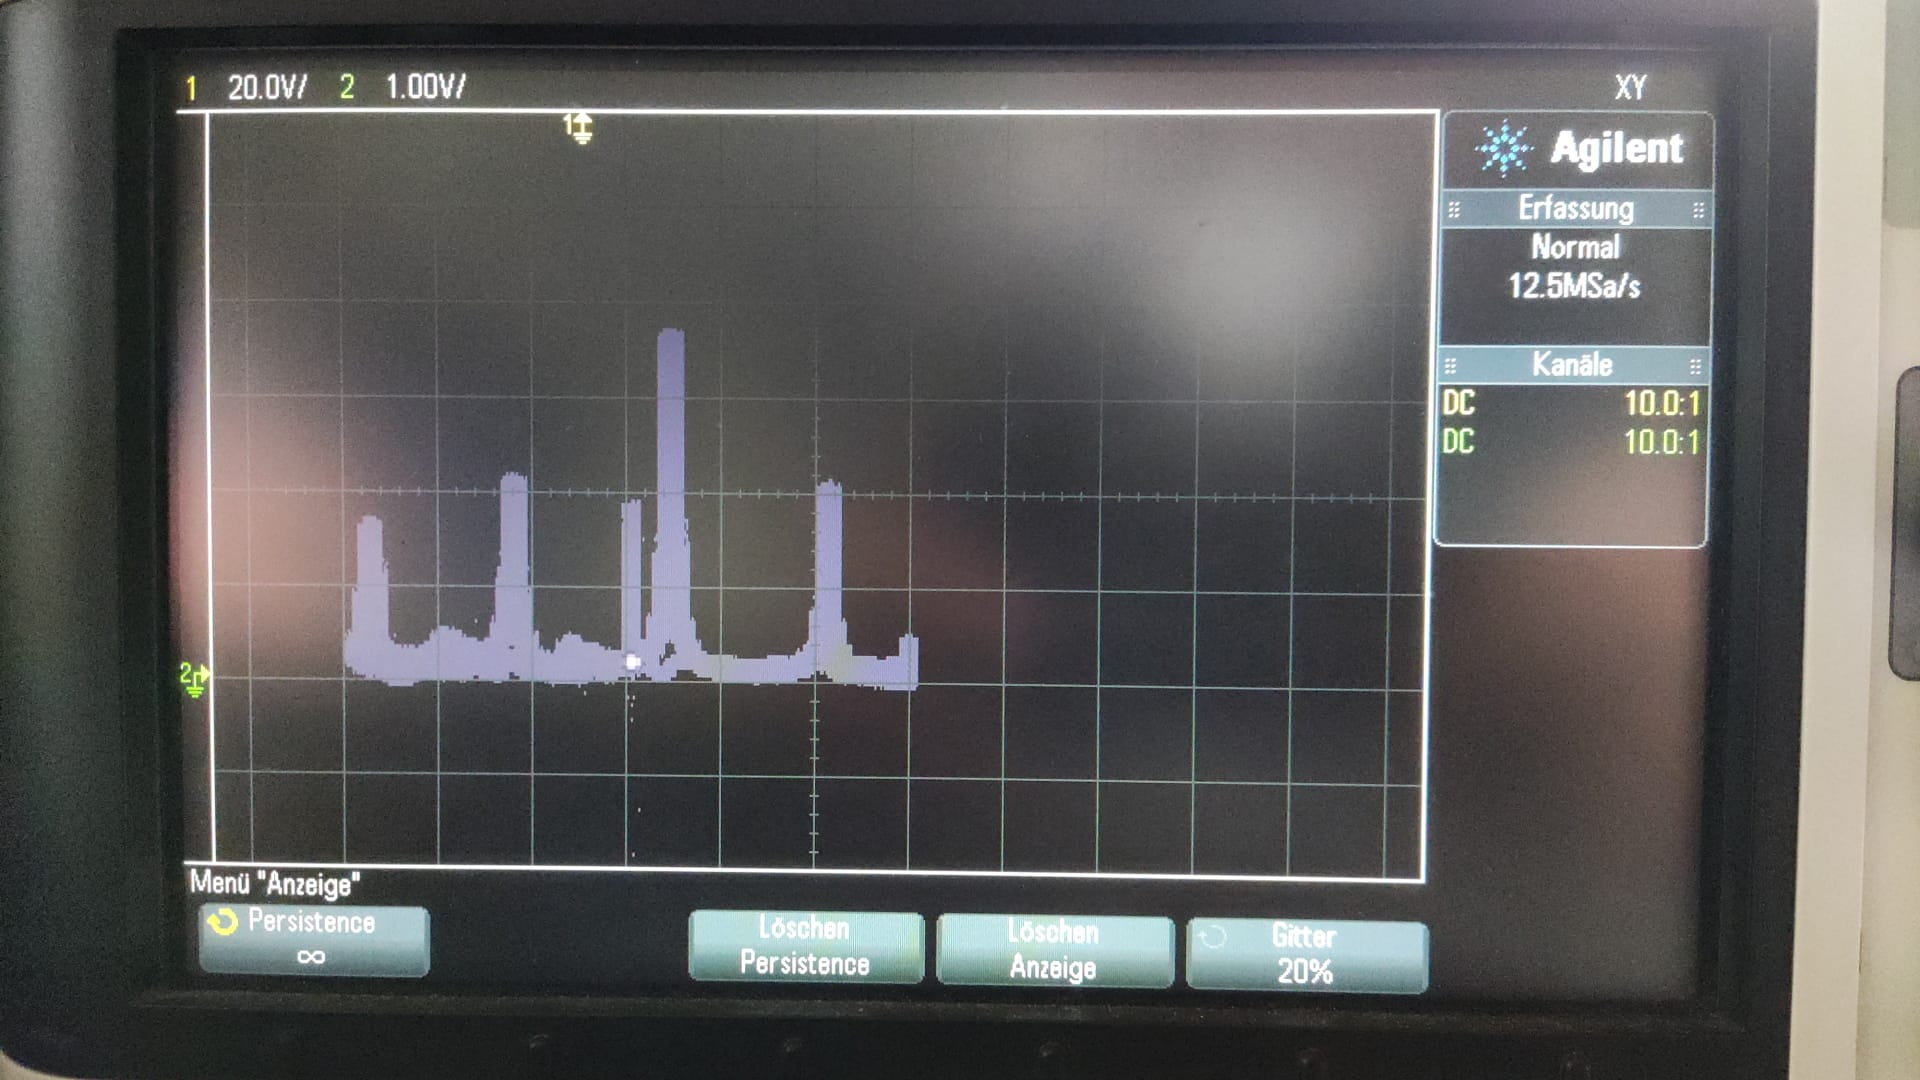
\includegraphics[height=3cm]{data_scripts/1.jpeg}%
\caption{Frequenzspektrum eines Zylinders mit der Länge $\qty{50}{\milli\meter}$}%
\label{fig:50os}%
\end{subfigure}%
\hfill% Fills available space in the center -> space between figures
\begin{subfigure}{0.48\textwidth}%
\centering%
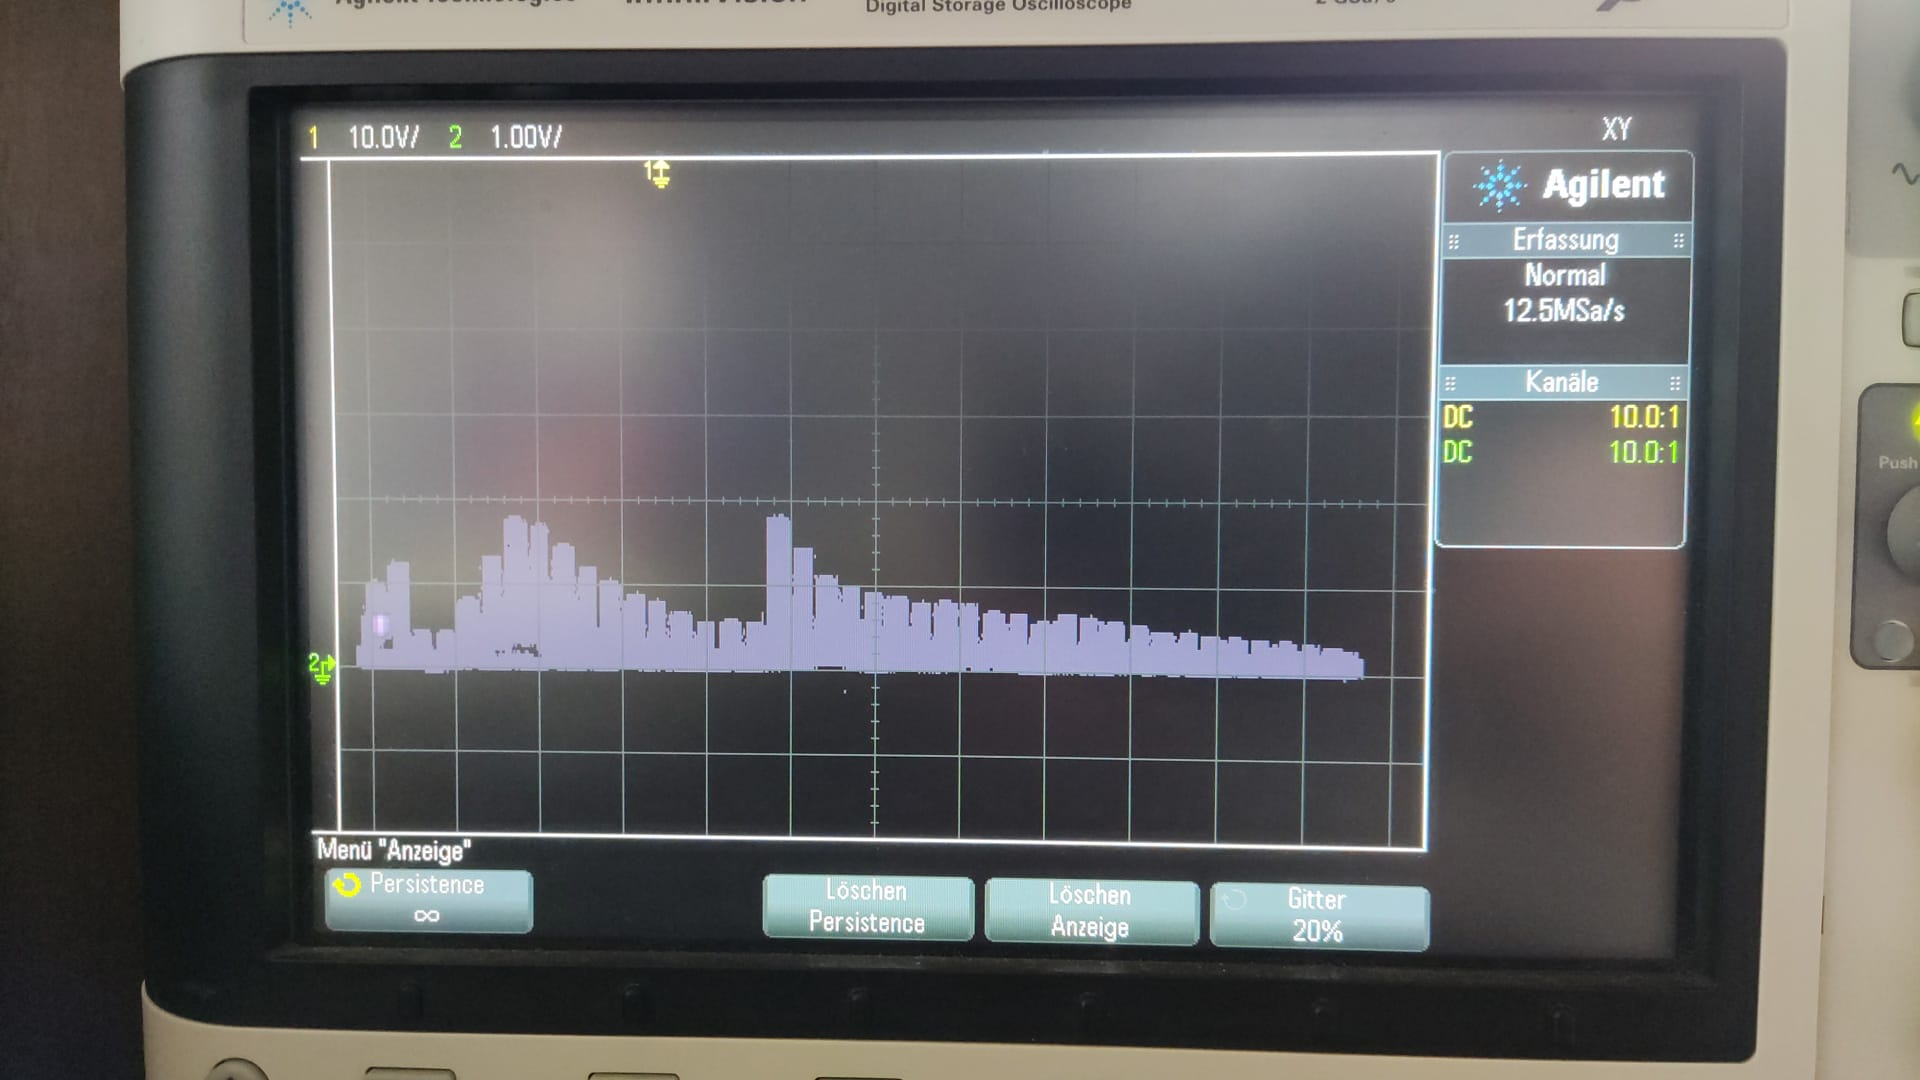
\includegraphics[height=3cm]{data_scripts/12.jpeg}%
\caption{Frequenzspektrum eines Zylinders mit der Länge $\qty{600}{\milli\meter}$}%
\label{fig:600os}%
\end{subfigure}%
\caption{Die Frequenzspektren von Zylindern mit jeweils $\qty{50}{\milli\meter}$ und $\qty{600}{\milli\meter}$, um die Frequenzspektren anderer Länge zu repräsentieren.}%
\label{fig:os}%
\end{figure}%


\subsection{Wasserstoffatom}
Um die Polarplots mit den Kugelflächenfunktionen zu vergleichen, wurden die Darstellungen dieser \cite{sphericalharmonics} entnommen.

\subsubsection{Hochaufgelöstes Frequenzspektrum bei sich gegenüberliegendem Mikrofon und Lautsprecher}
\begin{figure}
    \centering
    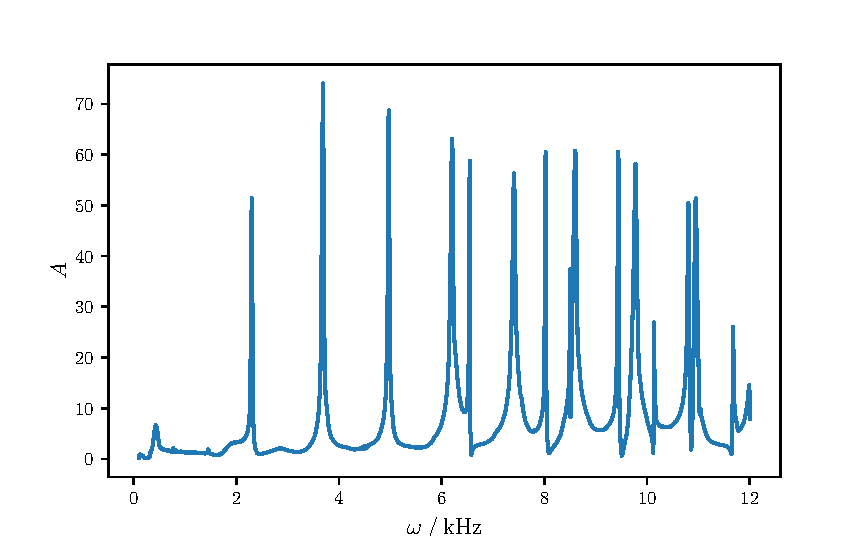
\includegraphics{build/hangle.pdf}
    \caption{Frequenzspektrum bei $\alpha = \ang{180}$}
    \label{fig:hangle}
\end{figure}
\FloatBarrier
In der Abbildung \ref{fig:600os} wird ersichtlich, dass sich die Peaks in der Abbildung \ref{fig:50os} zu mehreren kleineren Peaks aufspalten.

\subsubsection{Phasenverschiebung des aufgenommenen Welle}
Die relative Phase des oberen bzw. unteren Mikrofons $\varphi_{\symup{oben}}$ und $\varphi_{\symup{unten}}$ zur Eingangswelle ist für die jeweilige Resonanzfrequenz im Intervall 
$\omega \in [\qty{100}{\hertz}\, , \qty{10}{\kilo\hertz}]$ in Tabelle 
\ref{tab:hphase} angegeben. 
Ebenfalls ist die Phasenverschiebung $\symup{\Delta}\varphi = | \varphi_{\symup{oben}} - \varphi_{\symup{unten}} |$ angegeben
\begin{table}
    \centering
    \caption{Relative Phase zur Eingangswelle}
    \label{tab:hphase}
    \begin{tabular}{S[table-format=1.3] S[table-format=4] S[table-format=4] S[table-format=3]}
    \toprule
    {$\omega \mathbin{/} \si{\kilo\hertz}$} & $\varphi_{\symup{oben}}$ & $\varphi_{\symup{unten}}$ &{$\symup{\Delta}\varphi$} \\
    \midrule
        2.295   & 40    & 110   & 70 \\
        3.69    & -75   & 100   & 175\\
        6.24    & -40   & 33    & 73 \\
        7.43    & 0     & 180   & 180\\
        8.02    & 145   & -10   & 155\\
        8.64    & -180  & 6     & 185\\
        9.45    & -30   & -160  & 190\\
    \bottomrule
    \end{tabular}
  \end{table}

\subsubsection{Amplituden in Abhängigkeit des Winkels bei Resonanzfrequenzen}
In der Abbildung \ref{fig:hvarangle27} ist die Amplitude bei der Resonanzfrequenz $\omega = \qty{2.3}{\kilo\hertz}$, in Abbildung \ref{fig:hvarangle37} bei
$\omega = \qty{3.7}{\kilo\hertz}$, in Abbildung \ref{fig:hvarangle74} $\omega = \qty{2.3}{\kilo\hertz}$ und in Abbildung \ref{fig:hvarangle86} in Abhängigkeit 
des Winkels $\theta$ in einem Polarplot aufgetragen.
Der Winkel $\theta$ entspricht dabei nicht mit gemessenen Winkel $\alpha$. Zwischen den beiden Winkeln gilt die Beziehung 
\begin{equation}
    \theta = \arccos \left ( \frac{1}{2} \cos \left ( \alpha \right ) - \frac{1}{2} \right) \; {.}
\end{equation}
\begin{figure}
    \centering
    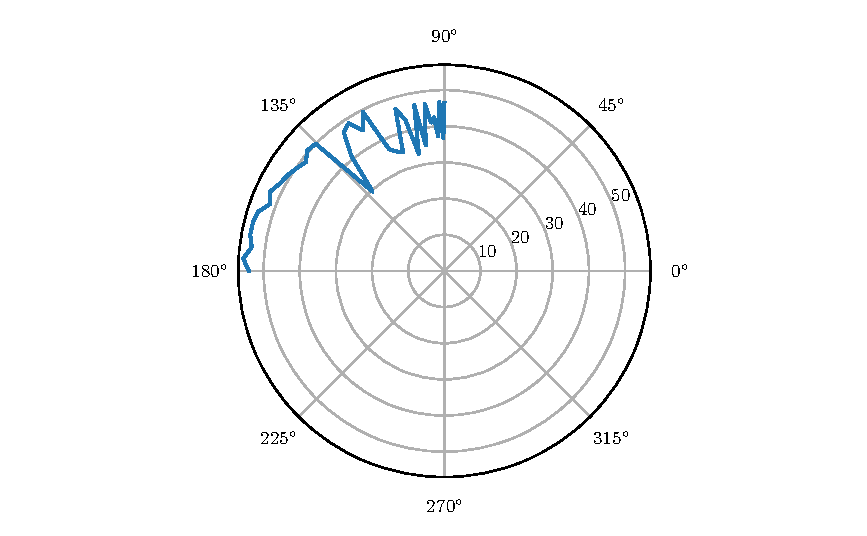
\includegraphics{build/hvarangle27.pdf}
    \caption{Polarplot des Peaks bei $\qty{2.3}{\kilo\hertz}$. Dies entspricht der Kugelflächenfunktion $Y_1^0$.}
    \label{fig:hvarangle27}
\end{figure}
\begin{figure}
    \centering
    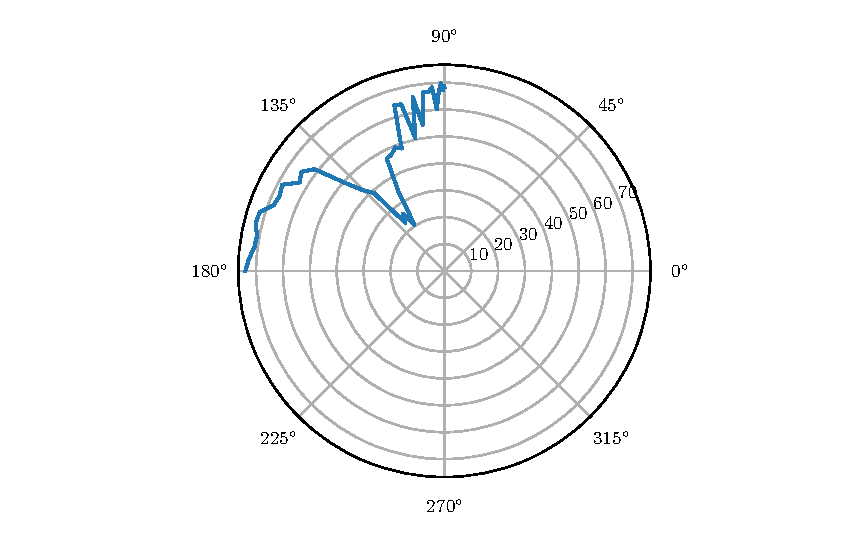
\includegraphics{build/hvarangle37.pdf}
    \caption{Polarplot des Peaks bei $\qty{3.7}{\kilo\hertz}$. Dies entspricht der Kugelflächenfunktion $Y_2^0$.}
    \label{fig:hvarangle37}
\end{figure}
\begin{figure}
    \centering
    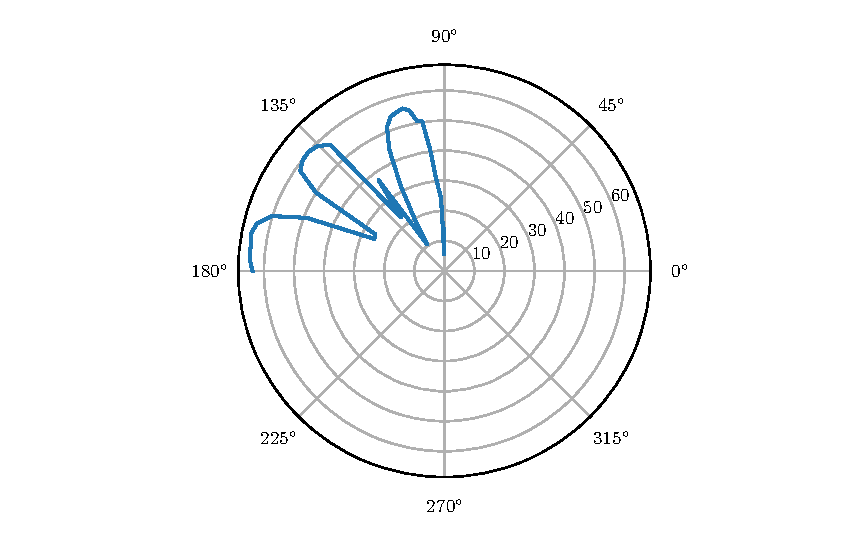
\includegraphics{build/hvarangle74.pdf}
    \caption{Polarplot des Peaks bei $\qty{7.4}{\kilo\hertz}$. Dies entspricht der Kugelflächenfunktion $Y_3^0$.}
    \label{fig:hvarangle74}
\end{figure}
\begin{figure}
    \centering
    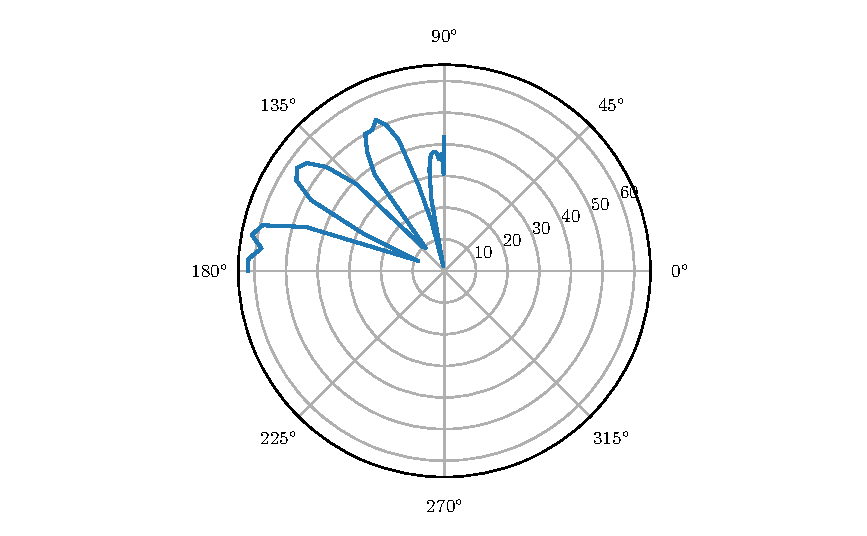
\includegraphics{build/hvarangle86.pdf}
    \caption{Polarplot des Peaks bei $\qty{8.62}{\kilo\hertz}$. Dies entspricht der Kugelflächenfunktion $Y_4^0$.}
    \label{fig:hvarangle86}
\end{figure}
\FloatBarrier

\subsubsection{Frequenzspektren bei Symmetriebrechung}
\begin{figure}
    \centering
    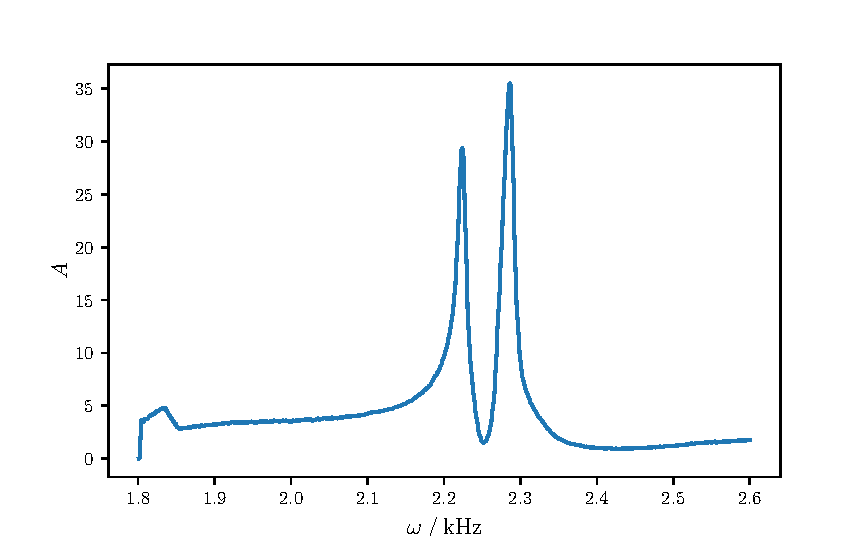
\includegraphics{build/h3ring.pdf}
    \caption{Frequenzspektrum des Wasserstoffatoms bei $\alpha = \ang{180}$ mit einem Zwischenring der Dicke $\qty{3}{\milli\meter}$.}
    \label{fig:h3ring}
\end{figure}
\begin{figure}
    \centering
    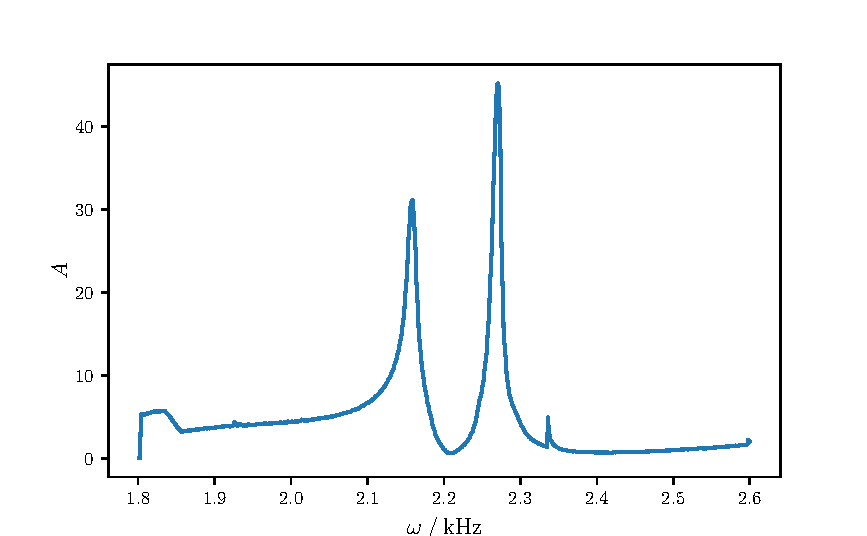
\includegraphics{build/h6ring.pdf}
    \caption{Frequenzspektrum des Wasserstoffatoms bei $\alpha = \ang{180}$ mit einem Zwischenring der Dicke $\qty{6}{\milli\meter}$.}
    \label{fig:h6ring}
\end{figure}
\begin{figure}
    \centering
    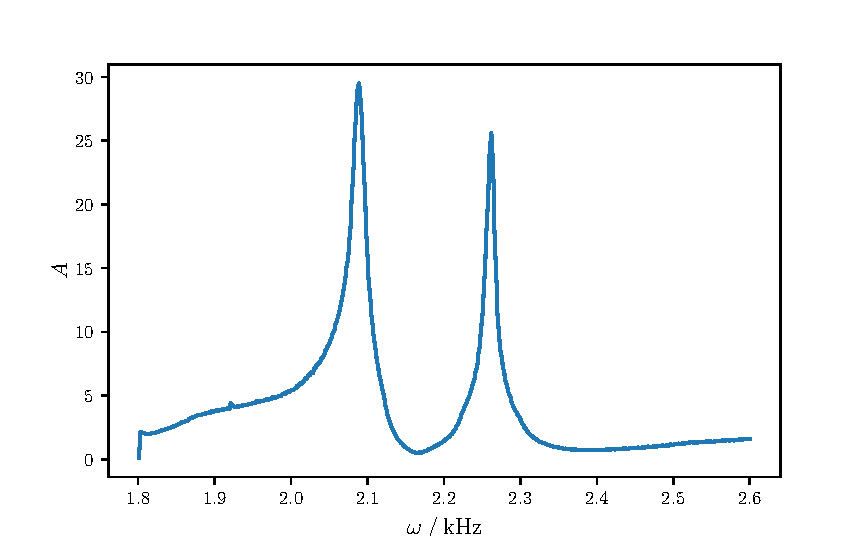
\includegraphics{build/h9ring.pdf}
    \caption{Frequenzspektrum des Wasserstoffatoms bei $\alpha = \ang{180}$ mit einem Zwischenring der Dicke $\qty{9}{\milli\meter}$.}
    \label{fig:h9ring}
\end{figure}
\FloatBarrier

\subsection{Wasserstoffmolekül}
\begin{figure}
    \centering
    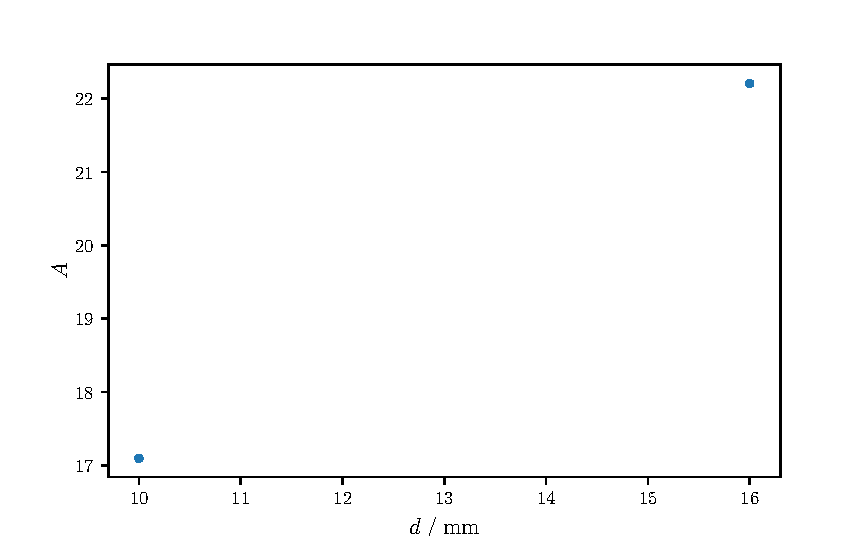
\includegraphics{build/h2dia.pdf}
    \caption{Resonanzamplitude des Wasserstoffmoleküls bei $\alpha = \ang{180}$ in Abhängigkeit des Blendendurchmessers.}
    \label{fig:h2dia}
\end{figure}
\begin{figure}
    \centering
    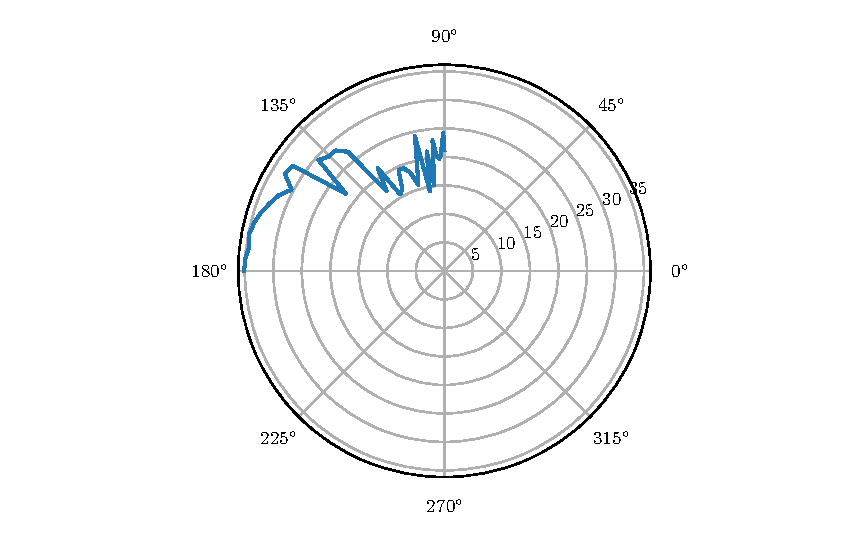
\includegraphics{build/h2varangle.pdf}
    \caption{Polarplot des Peaks bei $\qty{2.3}{\kilo\hertz}$.}
    \label{fig:h2varangle}
\end{figure}
\subsubsection{Phasenverschiebung}
\begin{table}
    \centering
    \caption{Relative Phase zur Eingangswelle}
    \label{tab:h2phase}
    \begin{tabular}{S[table-format=1.3] S[table-format=4] S[table-format=4] S[table-format=3]}
    \toprule
    {$\omega \mathbin{/} \si{\kilo\hertz}$} & $\varphi_{\symup{oben}}$ & $\varphi_{\symup{unten}}$ &{$\symup{\Delta}\varphi$} \\
    \midrule
        2.48   & 7    & -172   & 179 \\
        2.295  & 0    & 0      & 0\\
    \bottomrule
    \end{tabular}
  \end{table}
\subsection{1-dimensionaler Festkörper}
\begin{figure}
    \begin{subfigure}{0.48\textwidth}%
    \centering%
    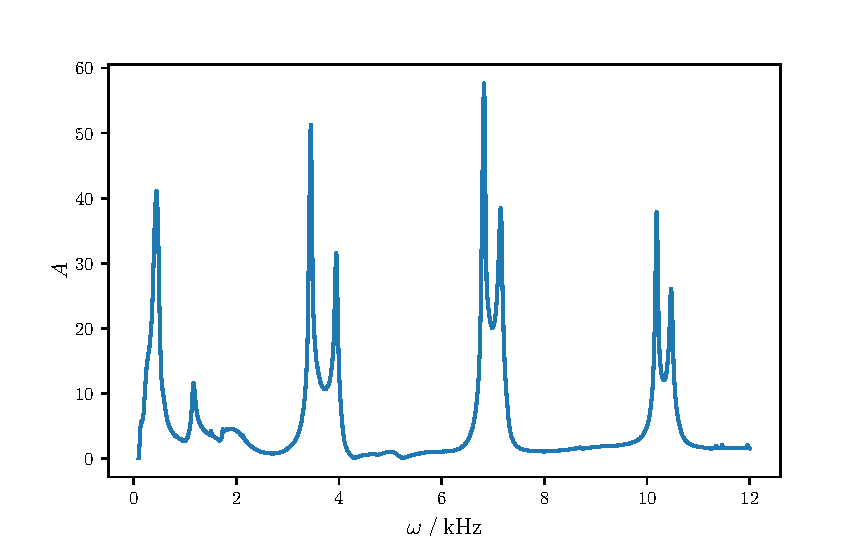
\includegraphics[height=5cm]{build/2c1b10.pdf}%
    \caption{Frequenzspektrum eines 1-dimensionalen Fesktörpers bestehend aus zwei $\qty{50}{\milli\meter}$ Zylindern und einer $\qty{10}{\milli\meter}$ Blende.}%
    \label{fig:2c1b10}%
    \end{subfigure}%
    \hfill% Fills available space in the center -> space between figures
    \begin{subfigure}{0.48\textwidth}%
    \centering%
    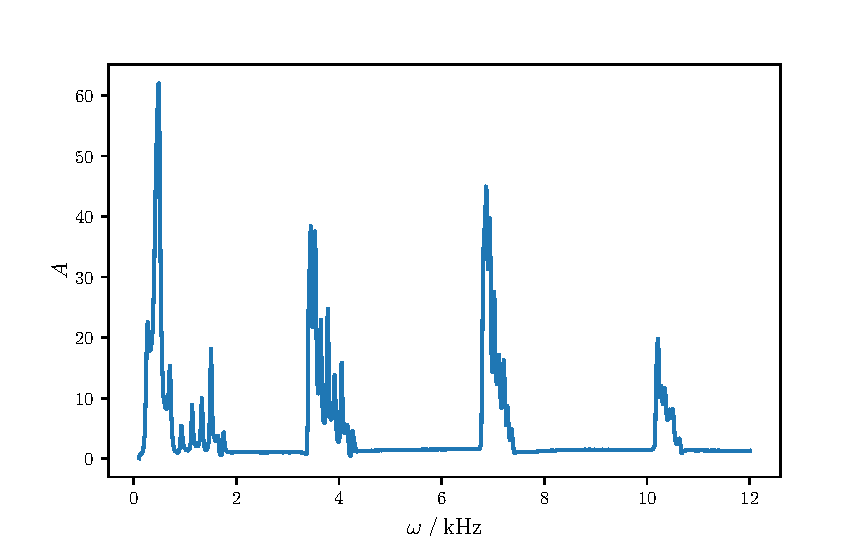
\includegraphics[height=5cm]{build/10c9b10.pdf}%
    \caption{Frequenzspektrum eines 1-dimensionalen Fesktörpers bestehend aus zehn $\qty{50}{\milli\meter}$ Zylindern und neun $\qty{10}{\milli\meter}$ Blenden.}%
    \label{fig:2c1b}%
    \end{subfigure}%
    \caption{Die Frequenzspektren von Festkörpern bestehend aus zwei bzw. zehn $\qty{50}{\milli\meter}$ Zylindern mit einer bzw. neun $\qty{10}{\milli\meter}$ Blenden, um die 
    Frequenzspektren der Festkörper, welche eine Länge zwischen diesen beiden Extrema haben, zu repräsentieren.}%
    \label{fig:10mm}
\end{figure}%
\begin{figure}
    \begin{subfigure}{0.48\textwidth}%
    \centering%
    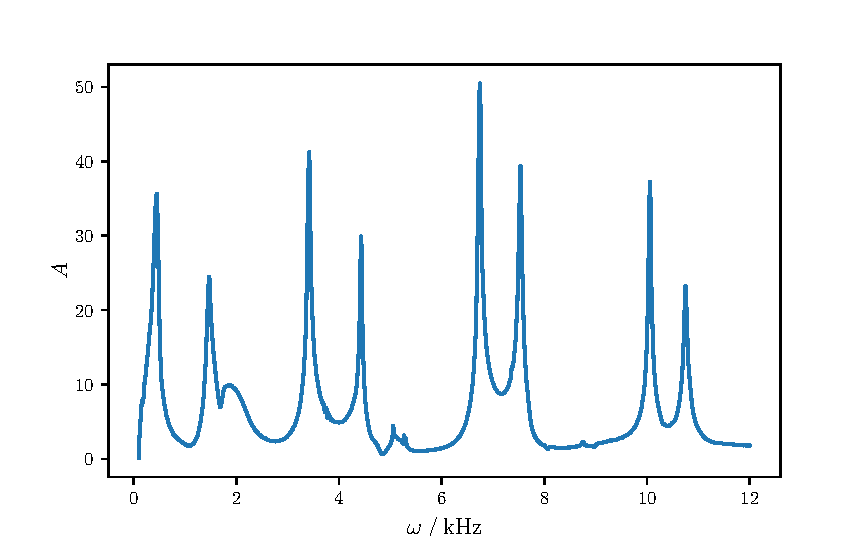
\includegraphics[height=5cm]{build/2c1b.pdf}%
    \caption{Frequenzspektrum eines 1-dimensionalen Fesktörpers bestehend aus zwei $\qty{50}{\milli\meter}$ Zylindern und einer $\qty{13}{\milli\meter}$ Blende.}%
    \label{fig:2c1b}%
    \end{subfigure}%
    \hfill% Fills available space in the center -> space between figures
    \begin{subfigure}{0.48\textwidth}%
    \centering%
    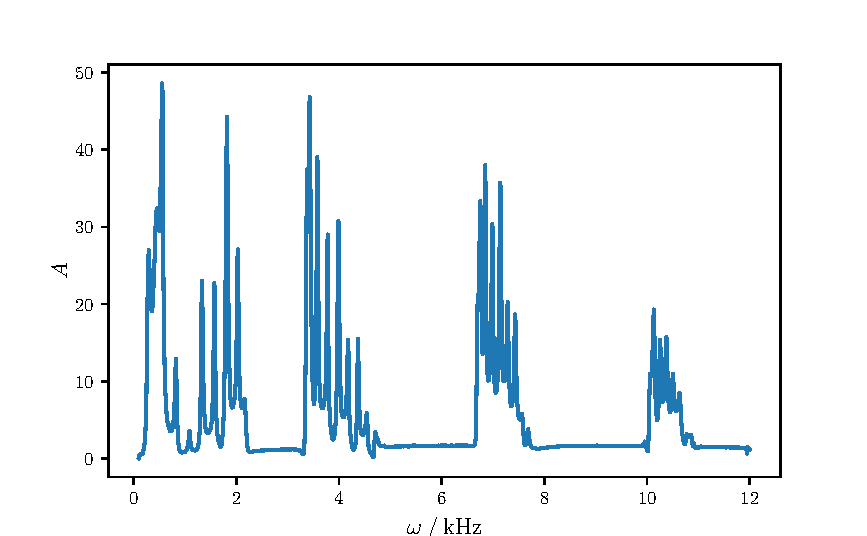
\includegraphics[height=5cm]{build/10c9b.pdf}%
    \caption{Frequenzspektrum eines 1-dimensionalen Fesktörpers bestehend aus zehn $\qty{50}{\milli\meter}$ Zylindern und neun $\qty{13}{\milli\meter}$ Blenden.}%
    \label{fig:2c1b}%
    \end{subfigure}%
    \caption{Die Frequenzspektren von Festkörpern bestehend aus zwei bzw. zehn $\qty{50}{\milli\meter}$ Zylindern mit einer bzw. neun $\qty{13}{\milli\meter}$ Blenden, um die 
    Frequenzspektren der Festkörper, welche eine Länge zwischen diesen beiden Extrema haben, zu repräsentieren.}%
    \label{fig:13mm}
\end{figure}%
\begin{figure}
    \begin{subfigure}{0.48\textwidth}%
    \centering%
    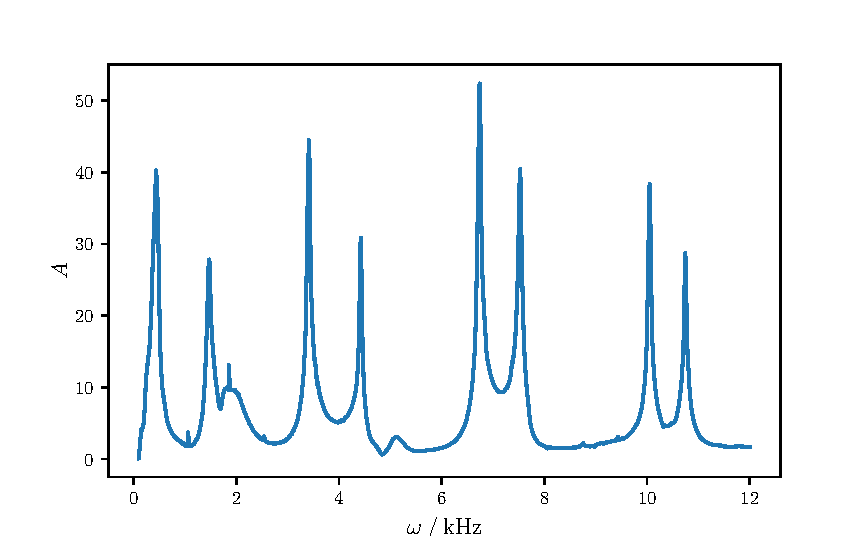
\includegraphics[height=5cm]{build/2c1b16.pdf}%
    \caption{Frequenzspektrum eines 1-dimensionalen Fesktörpers bestehend aus zwei $\qty{50}{\milli\meter}$ Zylindern und einer $\qty{16}{\milli\meter}$ Blende.}%
    \label{fig:2c1b16}%
    \end{subfigure}%
    \hfill% Fills available space in the center -> space between figures
    \begin{subfigure}{0.48\textwidth}%
    \centering%
    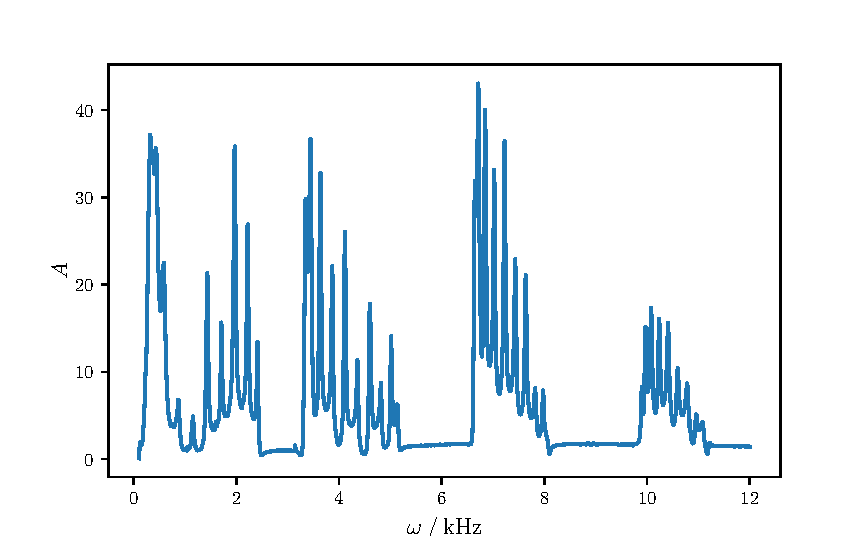
\includegraphics[height=5cm]{build/10c9b16.pdf}%
    \caption{Frequenzspektrum eines 1-dimensionalen Fesktörpers bestehend aus zehn $\qty{50}{\milli\meter}$ Zylindern und neun $\qty{16}{\milli\meter}$ Blenden.}%
    \label{fig:2c1b16}%
    \end{subfigure}%
    \caption{Die Frequenzspektren von Festkörpern bestehend aus zwei bzw. zehn $\qty{50}{\milli\meter}$ Zylindern mit einer bzw. neun $\qty{16}{\milli\meter}$ Blenden, um die 
    Frequenzspektren der Festkörper, welche eine Länge zwischen diesen beiden Extrema haben, zu repräsentieren.}%
    \label{fig:16mm}
\end{figure}%
\begin{figure}
    \begin{subfigure}{0.48\textwidth}%
        \centering%
        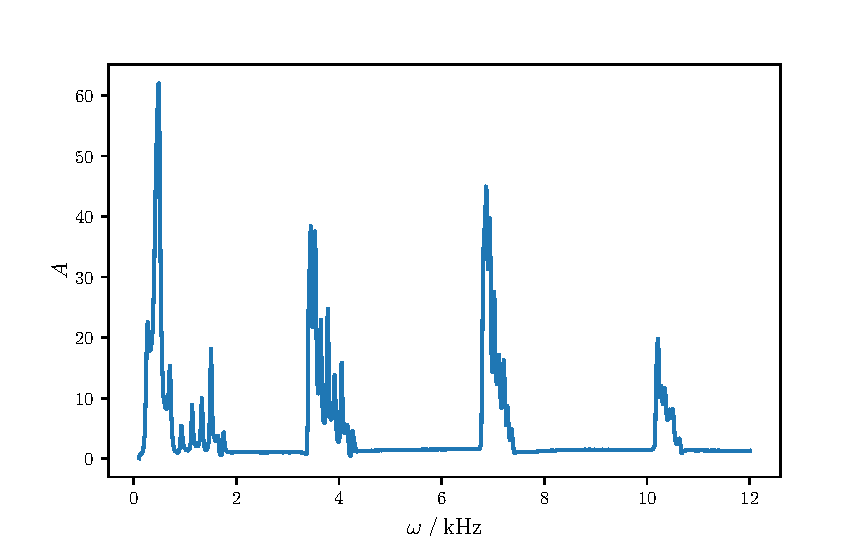
\includegraphics[height=5cm]{build/10c9b10.pdf}%
        \caption{Frequenzspektrum eines 1-dimensionalen Fesktörpers bestehend aus zwei $\qty{50}{\milli\meter}$ Zylindern und neun $\qty{10}{\milli\meter}$ Blenden.}%
        \label{fig:10c9b}%
    \end{subfigure}%
    \hfill% Fills available space in the center -> space between figures
    \begin{subfigure}{0.48\textwidth}%
        \centering%
        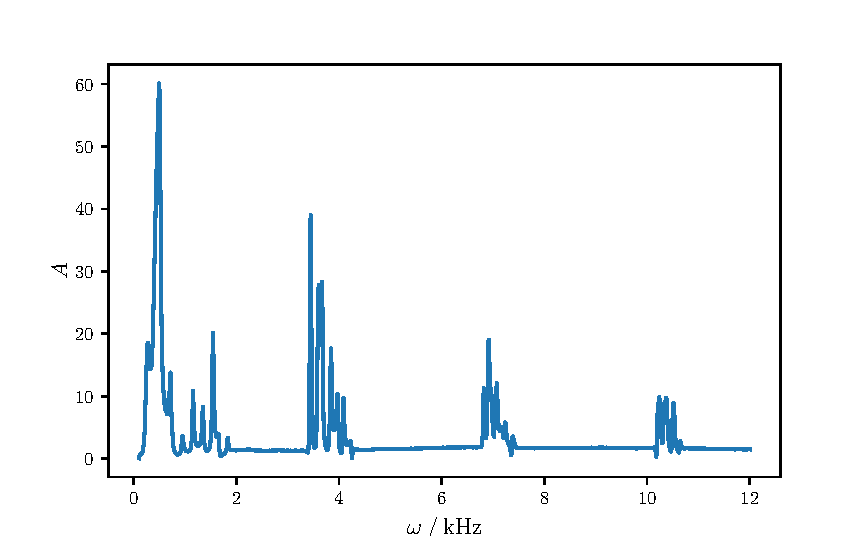
\includegraphics[height=5cm]{build/10c9b375.pdf}
        \caption{Frequenzspektrum eines 1-dimensionalen Fesktörpers bestehend aus neun $\qty{50}{\milli\meter}$ Zylindern, einem 
        $\qty{37.5}{\milli\meter}$ Zylinder und neun $\qty{10}{\milli\meter}$ Blenden.}%
        \label{fig:10c9b375}
    \end{subfigure} \\
    \begin{subfigure}{0.48\textwidth}%
        \centering%
        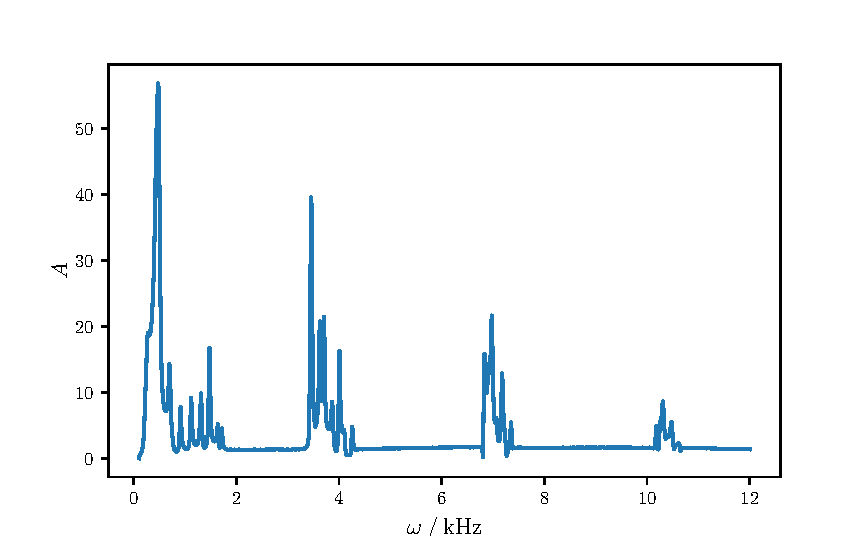
\includegraphics[height=5cm]{build/10c9b625.pdf}%
        \caption{Frequenzspektren eines 1-dimensionalen Fesktörpers bestehend aus neun $\qty{50}{\milli\meter}$ Zylindern, einem 
        $\qty{37.5}{\milli\meter}$ Zylinder und neun $\qty{10}{\milli\meter}$ Blenden.}%
        \label{fig:10c9b625}
    \end{subfigure}%
    \hfill
    \begin{subfigure}{0.48\textwidth}%
        \centering%
        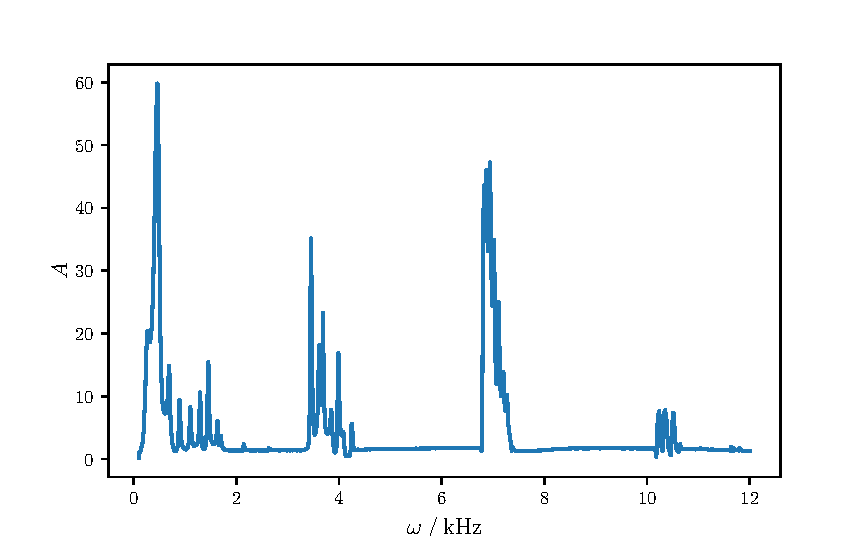
\includegraphics[height=5cm]{build/10c9b75.pdf}%
        \caption{Frequenzspektrum eines 1-dimensionalen Fesktörpers bestehend aus neun $\qty{50}{\milli\meter}$ Zylindern, einem 
        $\qty{625}{\milli\meter}$ Zylinder und neun $\qty{10}{\milli\meter}$ Blenden.}%
        \label{fig:10c9b75}
    \end{subfigure}%
    \caption{Die Frequenzspektren der Festkörper bestehend neun $\qty{50}{\milli\meter}$ Zylindern und einem variablen Zylinder mit neun $\qty{10}{\milli\meter}$ Blenden, um die 
            Frequenzspektren Festkörper, welche eine Länge zwischen diesen beiden Extremen haben, zu repräsentieren.}%
    \label{fig:austauschen}
\end{figure}%
\begin{figure}
    \centering
    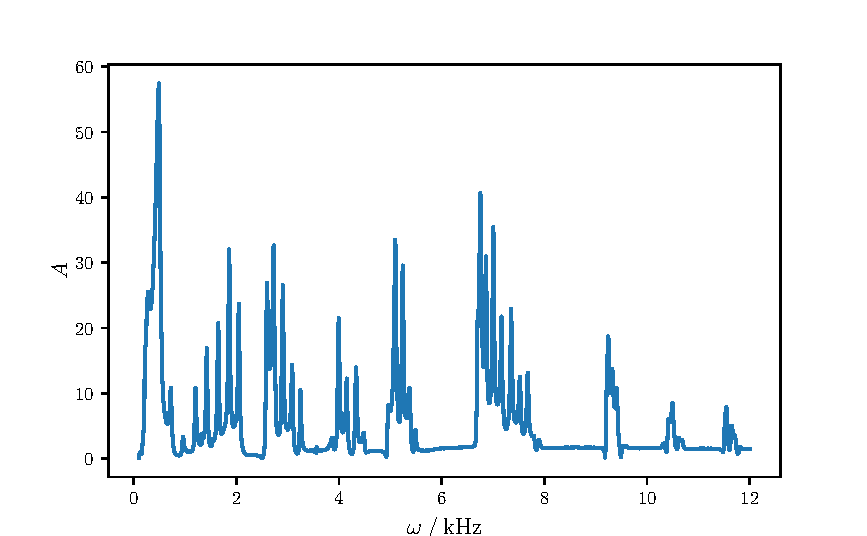
\includegraphics{build/5075.pdf}
    \caption{Frequenzspektrum eines Fesktörpers bestehend aus 10 alternierenden $\qty{50}{\milli\meter}$ und $\qty{75}{\milli\meter}$ mit neun 
    $\qty{16}{\milli\meter}$ Blenden.}
    \label{fig:5075}
\end{figure}
\begin{figure}
    \begin{subfigure}{0.48\textwidth}%
        \centering%
        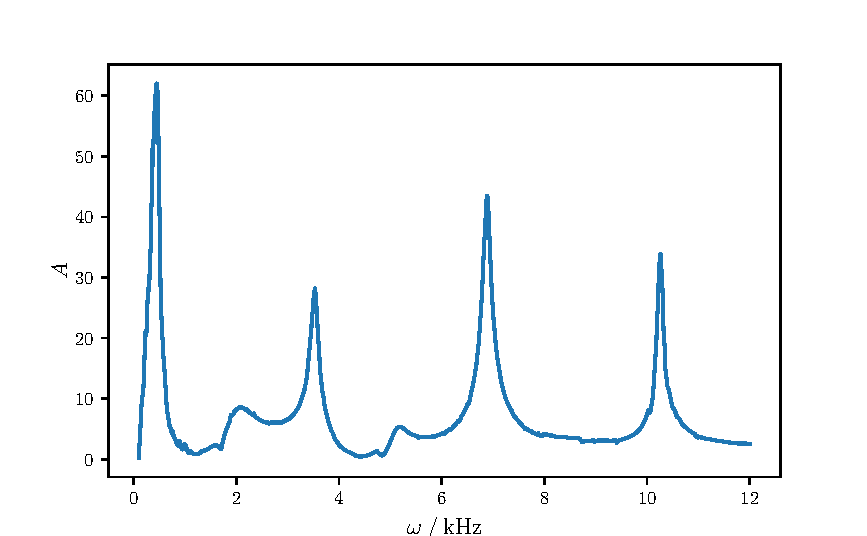
\includegraphics[height=5cm]{build/50single.pdf}%
        \caption{Frequenzspektrum von einem einzelnen $\qty{50}{\milli\meter}$ Zylinder.}%
        \label{fig:50sinlge}%
    \end{subfigure}%
    \hfill% Fills available space in the center -> space between figures
    \begin{subfigure}{0.48\textwidth}%
        \centering%
        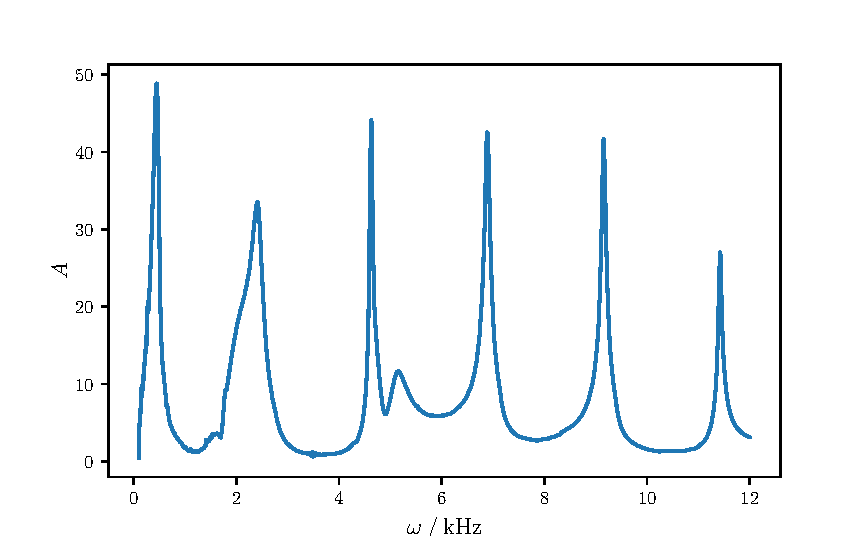
\includegraphics[height=5cm]{build/75single.pdf}%
        \caption{sFrequenzspektrum von einem einzelnen $\qty{75}{\milli\meter}$ Zylinder.}%
        \label{fig:75single}%
    \end{subfigure}%
    \caption{Die Frequenzspektren von einzelnen $\qty{50}{\milli\meter}$ bzw. $\qty{75}{\milli\meter}$ Zylindern, um diese mit dem Spektrum
    aus Abbildung \ref{fig:5075} zu vergleichen.}%
    \label{fig:75and50single}
\end{figure}%
\begin{figure}
    \centering
    \includegraphics{build/1316.pdf}
    \caption{Frequenzspektrum eines Festkörpers bestehend aus acht $\qty{50}{\milli\meter}$ Zylindern mit sieben alternierenden einzelnen $\qty{13}{\milli\meter}$ und 
    $\qty{16}{\milli\meter}$ Blenden.}
    \label{fig:1316}
\end{figure}